\begin{wrapfigure}{r}{2cm}
	\setbox0\hbox{
	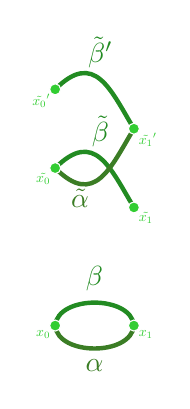
\begin{tikzpicture}
	%\clip (-0.2,-0.7) rectangle (1.2,4);
	%Definitionen
		\def\liftOfAlpha#1#2{
			\begin{scope}[yshift=#1cm]
				\draw[ultra thick, ForestGreen,] (0,0) .. controls (0.5,1) and (0.7,0) .. node[above]{\(#2\)} (1,-1);
			\end{scope}
		}
		\def\Anfangspunkte#1#2#3#4#5{
			\begin{scope}[xshift=#4cm,yshift=#1cm]
				\draw[fill=LimeGreen, draw= white, yscale=#3] (0,0) circle (2pt) node[below #5, LimeGreen, scale=0.5] {\(#2\)};
			\end{scope}
		}
		%Objekte unten
		\begin{scope}
			\draw[ultra thick, ForestGreen] (0,0) to[out=85,in=95] node[above] {\(\beta\)} (1,0);
			\draw[ultra thick, OliveGreen] (0,0) to[out=-85,in=-95] node[below] {\(\alpha\)} (1,0);

			%Punkte
			\Anfangspunkte{0}{x_0}{1}{0}{left}
			\Anfangspunkte{0}{x_1}{1}{1}{right}
			
			

		\end{scope}

		%Hochhebungen
		\begin{scope}[yshift=2cm, yscale= 0.5]
			\liftOfAlpha{0}{\tilde{\beta}}
			\liftOfAlpha{2}{\tilde{\beta}'}
			\draw[ultra thick, OliveGreen] (0,0) .. controls (0.5,-1) and (0.7,0) .. node[below left] {\(\tilde{\alpha}\)} (1,1);

			%hochgehobene Punkte
			\Anfangspunkte{0}{\tilde{x_0}}{2}{0}{left}
			\Anfangspunkte{2}{\tilde{x_0}'}{2}{0}{left}
			\Anfangspunkte{-1}{\tilde{x_1}}{2}{1}{right}
			\Anfangspunkte{+1}{\tilde{x_1}'}{2}{1}{right}
			\end{scope}
	\end{tikzpicture}	
	}\ht0=120pt
	\box0
\end{wrapfigure}